%%%%%%%%%%%%%%%%%%%%%%%%%%%%%%%%%%%%%%%%%%%%%%%%%%%%%%%%%%%%%%%%%%%%
\section{Overview}
\label{sec:fd-daq-ov}

\metainfo{DP/SP shared.  Georgia Karagiorgi and Dave Newbold. 2 Pages - largely
  generic but some highlighting of SP-specifics. 
  Focus on describing to HEP but non-DAQ expert. 
  Include how design is resilient in the face of potential
  uncertainties such as excess noise or the need to reduce drift HV
  (just two examples, maybe there are more).}

%%%%%%%%%%%%%%%%%%%%%%%%%%%%%%%%%
\subsection{Introduction}
\label{sec:fd-daq-intro}

The DUNE \dword{fd} \dword{daq} system must enable the readout,
triggering, processing and distribution to permanent storage of data
from all \dwords{detmodule} which includes both their electrical
\dword{tpc} and optical \dword{pds} signals.  
The final output data must retain, with very high efficiency and low
bias, a record of all activity in the detector which pertains to the
recognized Physics goal of the DUNE experiment. 
The practical constraints of managing this output requires that the
DAQ achieve these goals while reducing the input data volume by almost four
orders of magnitude.

The current generation of LArTPC DAQ, such as used in
\dword{protodune} and \microboone, record data over a fixed window of
time which is chosen based on the acceptance of an external trigger. 
The DUNE DAQ faces several major challenges beyond those of the
current generation. 
Foremost, it must accept data from about two orders of magnitude more
channels and from that data it must form its own triggers.
This self-triggering functionality requires immediate processing of
the full-stream data from a large portion of all TPC channels with a
throughput of approximately one terabyte per second per
\dword{detmodule}. 
From this data stream, triggers must be raised based on two very
different patterns of activity. 
The first is activity which is localized in a small region of one
\dword{detmodule} such as due to beam neutrino interactions or the
passage of relatively rare cosmic ray muons. 
This activity tends to correspond to relatively large deposition of
energy of around \SI{100}{\MeV} or more. 
The second pattern that must lead to a trigger lower energy activity
dispersed in time and spatial extent of the detector such as due to
\dword{snb}.

The DUNE \dword{fd} DAQ must also contend with a higher order of
complexity compared to current the generation. 
The \dword{fd} detector is not monolithic but ultimately will consist
of four \dwords{detmodule} each of \SI{10}{\kton} fiducial mass. 
Each module will follow somewhat unique technologies and the
inevitable asymmetries in the details of how data is read out from
each must be absorbed by the unified DAQ at its front-end. 
Further, each \dword{detmodule} is not monolithic but has at least one
layer of divisions, here generically named \dwords{detunit}. 
For example, the \dword{sp} \dword{detmodule} has \dwords{apa} each
providing data from a number of \dwords{wib} and the \dword{dp} has
\dword{cro} and \dword{lro} units associated with specific electronics
crates.
In each \dword{detmodule}, there are on order of 100 \dwords{detunit}
(150 for \dword{sp} and 245 for \dword{dp}) and each unit has a
channel count which of the same order as that of an entire LArTPC
detector of the current generation.
The DAQ, or really individual instances of the DAQ called
\dwords{daqpart}, must run on a subset of all possible
\dwords{detunit} for each given \dword{detmodule}. 
Each instance runs effectively independently from all others however
some instances will indirectly communicate through the exchange of
high level trigger information. 
This allows, for example, each \dword{detmodule} to take data in
isolation, for all to \dword{detmodule} to contribute to forming and
accepting global \dword{snb} triggers and simultaneously to have small
portions consisting of a few \dwords{detunit} running separately in
order to debug problems, run calibrations or otherwise not disturb
nominal data taking while maintaining high uptime.

Substantial computing hardware is required to provide the processing
capability needed to identify such activity while keeping up with the
rate of data.
The nature of various technical, financial and physical constraints
leads to much of the computing hardware needed to host this processing
to reside underground and near to the detector modules. 
In such an environment, power, cooling, space and access is far more
costly than typical data centers residing on the surface of the Earth.

Past LArTPC and long-baseline neutrino detectors have successfully
demonstrated external triggering using information related to their
associated particle beam. 
And indeed the DUNE FD DAQ will accept external information on recent
times of Main Injector beam spills from Fermilab. 
This will assure triggering with high efficiency to capture activity
pertaining to interactions from the produced neutrinos. 

However, even if the DUNE experiment had no physics goals other than
those related to neutrinos from these beam spills, an external beam
trigger alone is not sufficient. 
Absent any other information, such a trigger must inevitably call for
the readout of all possible data from the FD over a period of time of
at least as one LArTPC drift time. 
This would lead to an annual data volume approaching an exabyte
($10^{18}$ bytes) the vast majority of which consists of just noise. 
This entire data volume would have to be saved to permanent storage
and then processed offline in order to get to the signals.

Of course, DUNE does have a broad set of physics goals which expands
to include also the observation of interactions and decays that are
unrelated to the beam of neutrinos from Fermilab. 
This activity includes cosmic ray muons, which provide an important
source of detector calibration, and atmospheric neutrino interactions,
that give a secondary source from which to measure neutrino
properties. 
Taken together, and detailed below, recording their activity will
dominate the data rate.
The DAQ must also record data with sensitivity to rare interactions
(both known and hypothetical) such as nucleon decay, other baryon
number violating processes (such as neutron-antineutron oscillation),
and interactions from the products of \dwords{snb} as well as possibly
being able to observe isolated low energy interactions from solar
neutrinos and diffuse supernova neutrinos. 

Some of these events, while rare in themselves, produce patterns of
activity that can be mimicked by other higher rate backgrounds.
In the case of supernova neutrino bursts this is particularly so. 
While the exact processes involved in SNBs are not fully understood,
it is expected that a prolonged period of activity of many tens of
seconds will occur over which their neutrino interactions may be
observed. 
Individually, these interactions will be of low energy (relative to
that of beam neutrino interactions, for example) and will be spread
over time and the bulk of the \dwords{detmodule}. 
Because of their signature and their importance, special attention is
required to first ascertain that a SNB may be occurring and to save as
much data as possible over their duration.

Thus the DAQ must greatly reduce the full-stream of its input data
while using the data itself to do so. 
It must do this efficiently both in terms of recording essentially all
activity important to the physics goals of DUNE and in terms of
output data at a rate which is manageable.  


\subsection{Design Considerations}
\label{sec:fd-daq-des-consid}

The different \dwords{detmodule} have variation in terms of their
readout technology and schemes, timing system, channel counts and data
throughput and format.
All of this determines the nature of the digital data which is input
to the DAQ. 
The design of the DAQ strives to contain the unique layers which adapt
to the variation in \dwords{detmodule} toward its ``front end'' in
order to allow as many of its ``back end'' components identical across
the \dwords{detmodule} as possible. 
In particular, the DAQ must present a unified interface to the
ultimate consumer of its data, DUNE offline computing.
It must also accept and process the data from a variety of other
sources including the accelerator, various calibration systems
(including laser, cold electronics, photodetectors, and potentially
others) as well as trigger sources external to DUNE. 
The daq must be optimized for the above while also retaining
flexibility to scale to handle certain risks such as excess noise,
changes in high voltage, cut network connectivity and other credible
potentialities.

\begin{dunefigure}[DAQ Overview]{fig:daq-overview}
  {The high-level, nominal design for the DUNE FD DAQ showing data (solid, with
    line width indicating throughput) and trigger (dashed) flows. 
    A detector module has specialized implementation of some of these
    high level components, particularly toward the upstream front-end
    as described in the text. 
    The grayed boxes are not in the DAQ scope.
    See text for details.
}
% This PDF is made from the .dot of the same name.
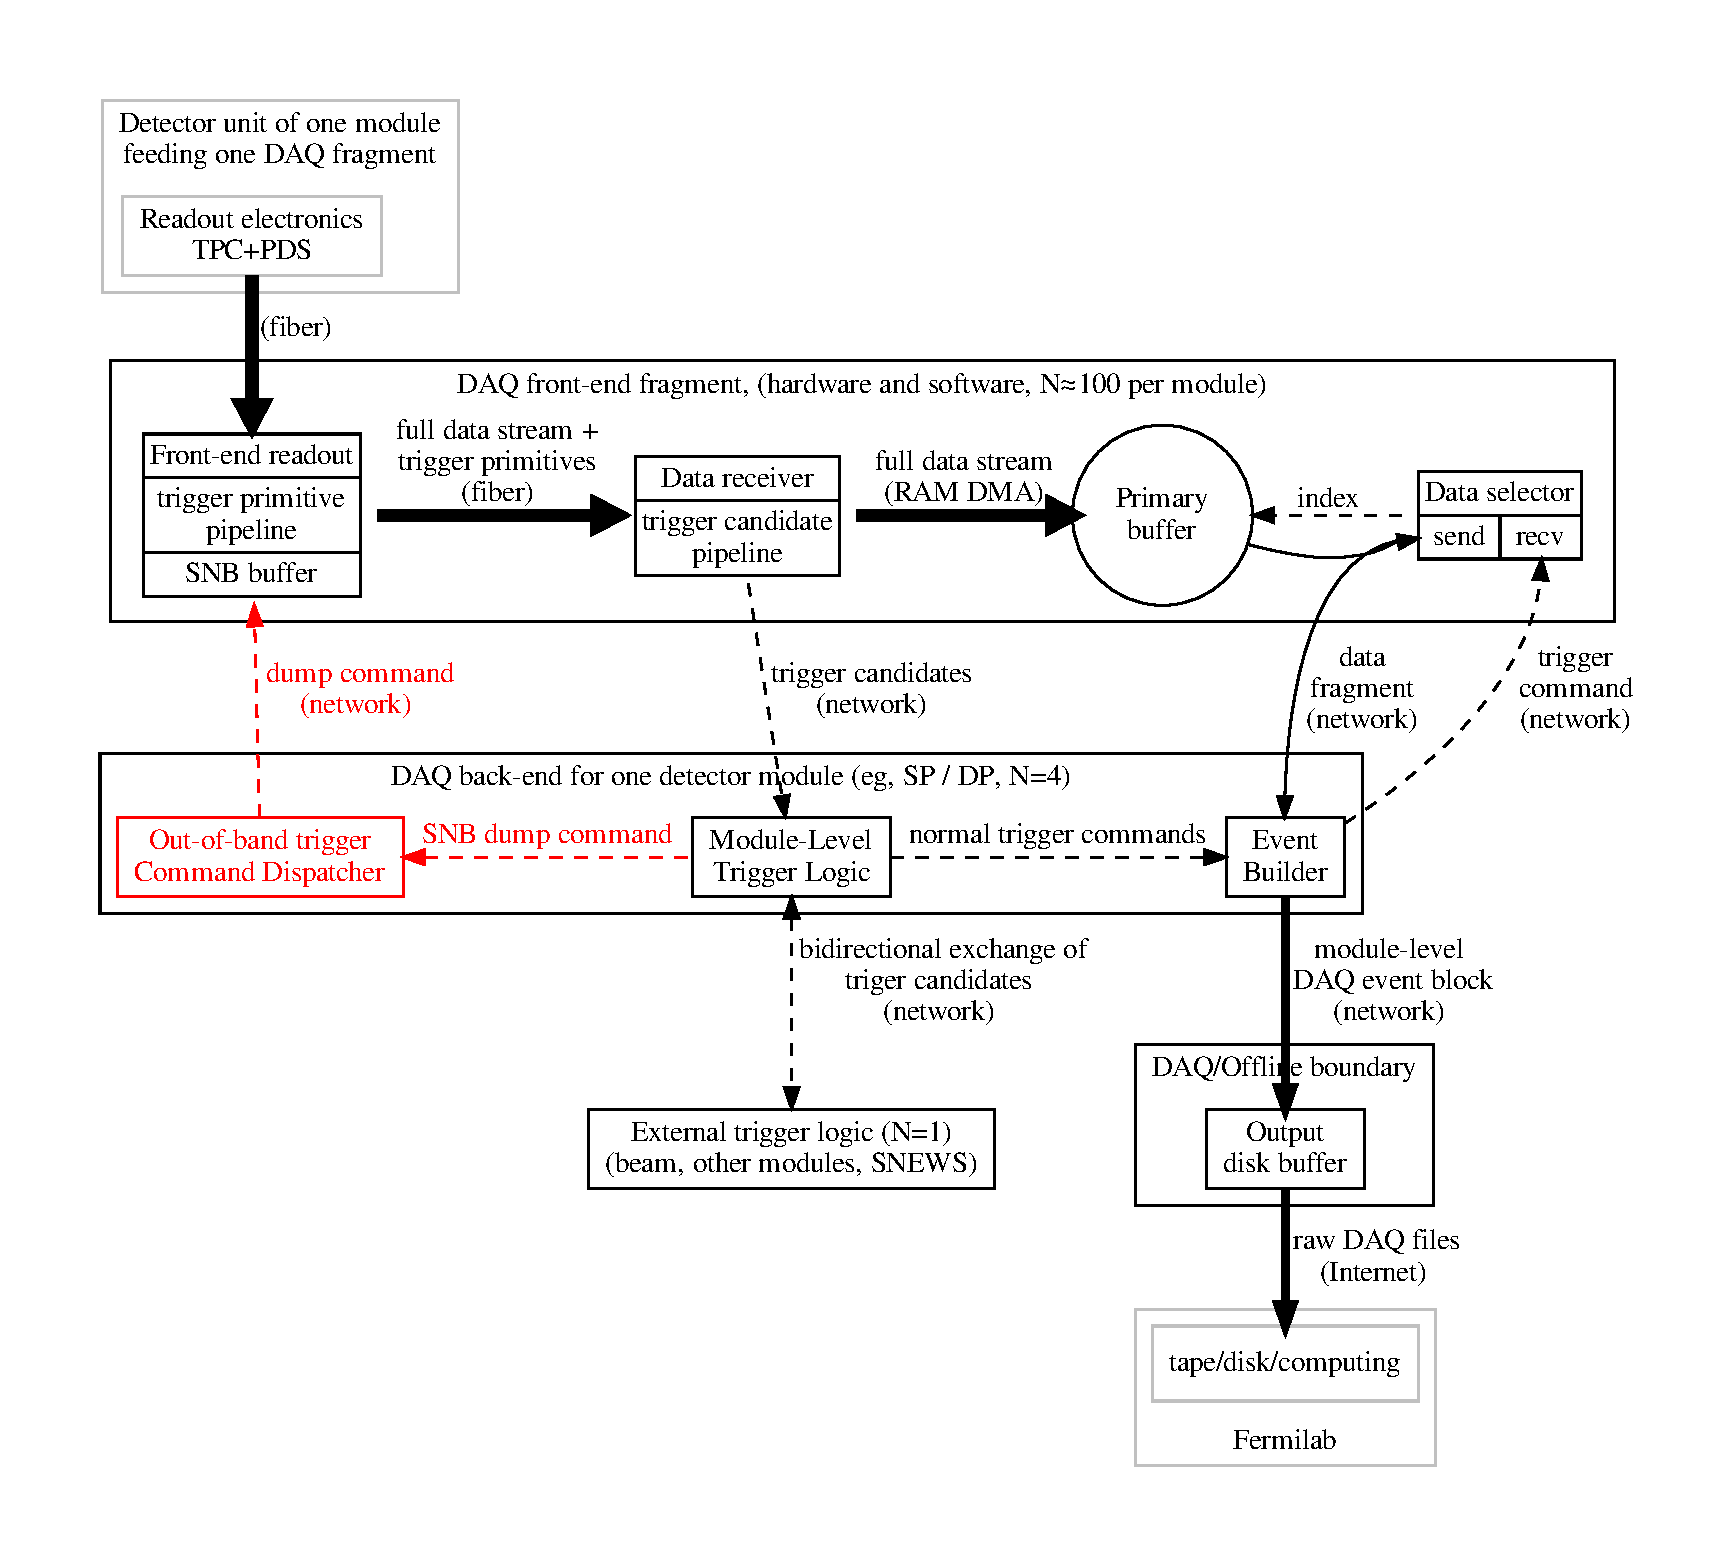
\includegraphics[width=0.8\textwidth]{high-level-daq.pdf}%
\end{dunefigure}

\begin{dunefigure}[DAQ Overview]{fig:daq-overview-alt}
  {The high-level, alternative design for the DUNE FD DAQ showing data (solid, with
    line width indicating throughput) and trigger (dashed) flows. 
    A detector module has specialized implementation of some of these
    high level components, particularly toward the upstream front-end
    as described in the text. 
    The grayed boxes are not in the DAQ scope.
    See text for details.
}
% This PDF is made from the .dot of the same name.
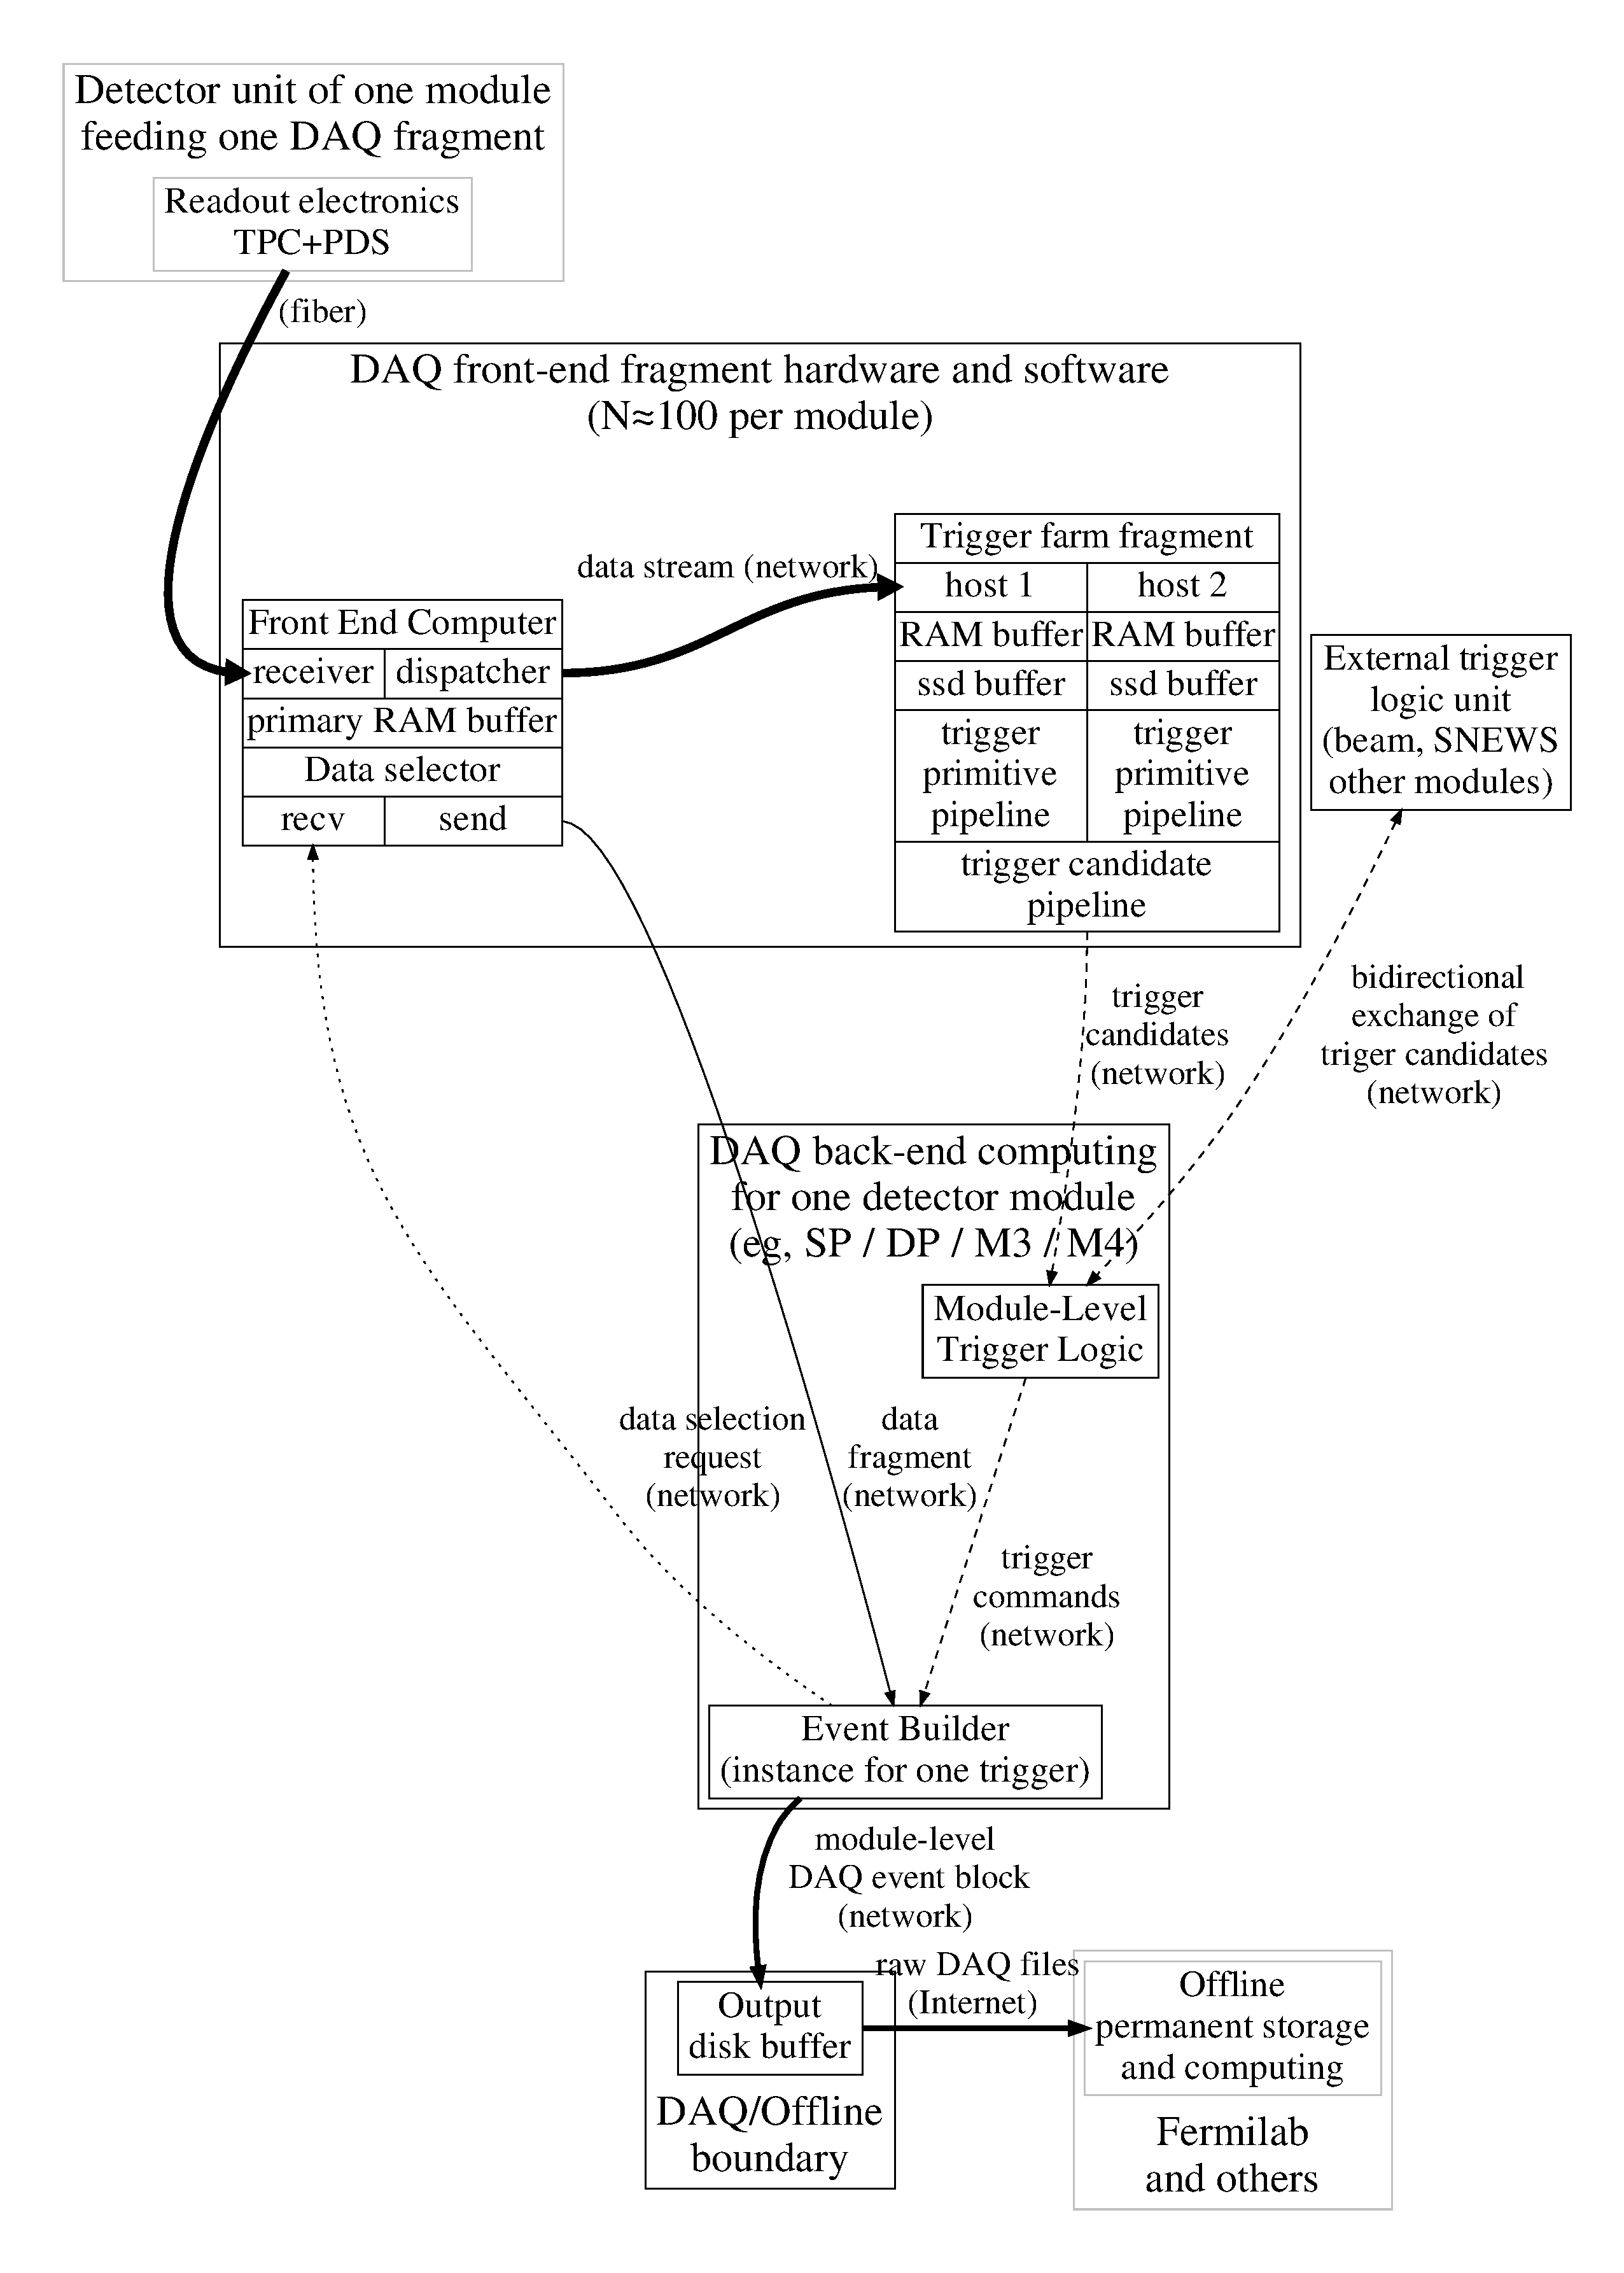
\includegraphics[width=0.8\textwidth]{high-level-daq-alt.pdf}%
\end{dunefigure}

Currently, two major variations for the DUNE DAQ are considered. 
They differ at their front-ends and in terms of the order in which
they buffer the data after it is received from the detector
electronics and in which they use that data to form
\dwords{trigprimitive}.
The first design, designated as nominal, forms \dwords{trigprimitive}
before the data reaches the DAQ \dword{ringbuffer}. 
In a high-level way, it is illustrated in Fig~\ref{fig:daq-overview}
in terms of data and trigger flows.
The second, designated as alternative, reverses this order and is
illustrated in Fig~\ref{fig:daq-overview-alt}. 
These high level diagrams and their design are described in
detail in Section~\ref{sec:fd-daq-overview}.

At their level of detail the two diagrams are generic to all
\dwords{detmodule} but some of the depicted roles will necessarily
have implementation specific to their \dword{detmodule}.
The subsections of Section~\ref{sec:fd-daq-design} give more
description of this high-level design as well as details on
specialized implementations in particular see
Sections~\ref{sec:fd-daq-fero} and~\ref{sec:fd-daq-fetp} which
describe specializations of the front end required to adapt to the SP
and DP \dwords{detmodule}.

The high level requirements for the DUNE FD DAQ are provided in
\cite{daq:reqs}.
The most critical requirements in consideration for the overall design
are summarized in Table~\ref{tab:daqrequirements}.

\begin{dunetable}[Important requirements on the DAQ system design]
{p{0.2\textwidth}p{0.6\textwidth}}
{tab:daqrequirements}
{Important requirements on the DAQ system design}   
Requirement  & Description \\ \toprowrule
Scalability & The DUNE FD DAQ shall be capable of receiving and
buffering the full raw data from all four FD modules \\ \colhline 
Zero deadtime & The DUNE FD DAQ shall operate without deadtime under
"normal" operating conditions \\ \colhline
Triggering & The DUNE FD DAQ shall provide full-detector triggering
functionality as well as self-triggering
functionality; the data selection shall maintain high efficiency to
physics events while operating within a total bandwidth of \offsitepbpy
for all operating FD modules \\ \colhline
Synchronization & The DUNE FD DAQ will provide synchronization of
different FD modules to within 1~$\mu$s, and of different subsystems
within a module to within 10~ns\\ \colhline
\end{dunetable}

The input bandwidth and processing needs of the DAQ are expected to be
dominated by the rate of data produced by the TPC system of each
\dword{detmodule}.
These rates vary between the modules and their estimations are summarized in
Table.~\ref{tab:daq-input-bandwidth}.
\begin{dunetable} [Pre-trigger data rates from the DUNE FD TPCs and
  into DAQ front end.]
  {lll} {tab:daq-input-bandwidth} {The parameters governing the
    pre-trigger data rate from units of each \dword{detmodule} TPC
    \dwords{ce} and the aggregate throughput into the \dwords{fec} of
    the DAQ \dwords{daqfrag}. 
    Compression is an estimate and will be reduced if excess noise is
    introduced.  
  }
  parameter & \dlong{sp} & \dlong{dp} \\
  \colhline
  TPC unit & APA & CRO crate \\
  unit multiplicity & 150 & 240 \\
  channels per unit & 2560 (800 collection) & 640 (all collection) \\
  ADC sampling & \SI{2}{\MHz} & \SI{2.5}{\MHz} \\
  ADC resolution & 12 bit & 12 bit \\
  \colhline
  aggregate from \dword{ce} & \SI{1440}{\GB/\s} & \SI{576}{\GB/\s} \\
  with compression & \SI{230}{\GB/\s} (5$\times$) & \SI{58}{\GB/\s} (10$\times$)  \\
  \colhline
\end{dunetable}

The ultimate limit on the output data rate of the DUNE FD DAQ is
expected to be provided by the available bandwidth to and the tape,
disk and processing capacity of Fermilab. 
An ample guideline has been established which places this limit at
about \offsitepbpy or \offsitegbps.
Extrapolating to four FD detector modules this requires the DAQ to
perform a data reduction factor of almost four orders of magnitude. 
This will be achieved through a simple self-triggered readout strategy.

An overestimate of the annual, triggered but uncompressed data volume
for one \SI{10}{\kton} \dword{detmodule} is summarized in
Table.~\ref{tab:daq-data-rates}. 
It assumes a very generous and simple trigger scheme whereby the data
from the entire \dword{detmodule} is saved for a period longer than
two drift times around the trigger time.
This will essentially remove any selection bias at the cost of
recording a substantial amount of data that will simply contain noise.

\begin{dunetable} [Uncompressed data rates for one SP module.]
  {p{0.30\textwidth}p{0.13\textwidth}p{0.4\textwidth}}
  {tab:daq-data-rates} {Anticipated anual, uncompressed data rates
    for a single SP module. The rates for normal (non-SNB triggers)
    assume a readout window of \SI{5.4}{\ms}. 
    For planning purposes these rates are assumed to apply to the DP
    module as well which has a longer readout time but fewer channels. 
    In reality, lossless compression will be applied which is expected
    to provide as much as a $5\times$ reduction in data volume for the SP module
    and as much as $10\times$ for the DP module.}   
  Event Type  & Data Volume \si{\PB/year} & Assumptions \\ \toprowrule
  Beam interactions & 0.03 & 800 beam and 800 dirt muons; \SI{10}{\MeV} threshold in coincidence with beam time; include cosmics\\ \colhline
  Cosmics and atmospherics & 10 &  \SI{10}{\MeV} threshold, anti-coincident with beam time \\ \colhline
  Radiologicals & $\le$1 & fake rate of $\le$100 per year \cite{daq:simreport}\\ \colhline
 Front-end calibration & 0.2 & Four calibration runs per year, 100 measurements per point \\ \colhline
 Radioactive source calibration & 0.1 & source rate $\le$10~Hz; single APA readout; lossless readout \\ \colhline
 Laser calibration & 0.2 & 1$\times$10$^6$ total laser pulses, lossy readout \\ \colhline
 Supernova candidates & 0.5 & 30 seconds full readout, average once per month \\ \colhline
 Random triggers & 0.06 & 45 per day\\ \colhline
 Trigger primitives & $\le$6 &  all three wire planes; 12 bits per primitive word; 4 primitive quantities; $^{39}$Ar-dominated\\ \colhline
\end{dunetable}

The data volume estimates also assume that any excess noise beyond
what is expected due to intrinsic electronics noise will not lead to
an increase in trigger rates. 
If, for example, excess noise occurs such that it frequently mimics
more than about \SI{10}{\MeV} of localized ionization then this would
lead to an increase in various types of triggers and subsequently more
data.
However, at the same time, these estimates do not take into account
that some amount of lossless compression of the TPC data will be
achieved. 
In the absence of excess noise it is expected that a compression
factor of at least $5\times$ can be achieved with the SP data and up
to $10\times$ may be achieved with the DP data. 
Of course, the compression factor achieved will ultimately depend on
the level of excess noise experienced in each \dword{detmodule}
cryostat. 
Studies using data from the LBNE 35t prototype and early MicroBooNE
running have shown that a compression factor of at least $4\times$ can
be expected even in the case of rather high levels of excess noise.

One category that will be particularly sensitive to excess noise will
be the trigger primitives. 
As discussed more in Section~\ref{sec:fd-daq-fetp}, their primary
intended use are as transient objects produced and consumed locally
and directly by the DAQ in the \dword{trigdecision} process. 
However, as their production is expected to be dominated by $^{39}$Ar
decays (absent excess noise) they may carry information that proves
very useful for calibration purposes. 
Future studies with simulation and with early data will determine what
are the most feasible methods to exploit this data. 
These may include committing all or a portion to permanent storage or
potentially developing processes that can summarize their data while
still retain information salient to calibration.

Finally, it is important to note that early data will be used to
evaluate other selection criteria. 
It is expected that efficient and bias free selections can be
developed and validated which save a subset of the entire
\dword{detmodule} for any given trigger type. 
For example, a cosmic muon trigger command will indicate which APAs
contributed to its formation (which had local ionization activity). 
This command can then direct reading out these APAs, possibly also
including their neighbors while discarding the data from all other
APAs. 
This may reduce the estimated \SI{10}{\PB/year} for ``cosmics and
atmospherics'' by an order of magnitude. 
A similar advanced scheme can be applied the \dword{dp}
\dword{detmodule} by retaining data for the given readout window from
only the subset of \dword{cro} crates (and again, potentially their
nearest neighbors) which contributed to the formation of the given
trigger.



%%%%%%%%%%%%%%%%%%%%%%%%%%%%%%%%
\subsection{Scope}
\label{sec:fd-daq-scope}

%\metainfo{This section may also wish to refer to Fig.~\ref{fig:daq-overview}.}

The nominal scope of the \dword{daq} system is illustrated in
Fig.~\ref{fig:daq-overview} by the boxes which are not grayed out and
includes the continued procurement of materials for, and the
fabrication, testing, delivery and installation of the following
systems:

\begin{itemize}
\item Front-end readout (nominal design) or trigger farm (alternative
  design) hardware and firmware or software development for
  \dword{trigprimitive} generation.
\item Front-end computing for hosting of \dword{daqdr}, \dword{ringbuffer} and \dword{daqds}.
\item Back-end computing for hosting \dword{mtl}, \dword{eb} and the \dword{daqoob} processes.
\item External trigger logic and its host computing.
\item Algorithms to generate trigger commands which perform data selection.
\item Timing distribution system
\item DAQ data handling software including receiving and building of
  events
\item Run control software, configuration database, and user interface
\item Rack infrastructure in the central utility cavern for readout
  electronics, front-end computing, timing distribution, and data
  selection
\item Rack infrastructure on surface at SURF for back-end computing
\end{itemize}
